\section{First-Order Partial Derivatives} \label{S:10.2.First_Order_Partial_Derivatives}

\vspace*{-14 pt}
\framebox{\hspace*{3 pt}
\parbox{6.25 in}{\begin{goals}
\item How are the first-order partial derivatives of a function $f$ of
  the independent variables $x$ and $y$ defined?  
\item Given a function
  $f$ of the independent variables $x$ and $y$, what do the first-order partial derivatives $\frac{\partial
    f}{\partial x}$ and $\frac{\partial f}{\partial y}$ tell us about $f$?
\end{goals}} \hspace*{3 pt}}


\subsection*{Introduction}

The derivative plays a central role in first semester  calculus
because it provides important information about a function.  Thinking
graphically, for instance, the derivative at a point tells us the
slope of the tangent line to the graph at that point.  In addition, the
derivative at a point also provides the instantaneous rate of change of
the function with respect to changes in the independent variable.

Now that we are investigating functions of two or more variables, we
can still ask how fast the function is changing, though we have to be careful about what we mean.  Thinking
graphically again, we can try to measure how steep the graph of the
function is in a particular direction.  Alternatively, we may want to know how fast a function's
output changes in response to a change in one of the inputs.
Over the next few sections, we will develop tools for addressing
issues such as these these.  Preview
Activity \ref{PA:10.2} explores some issues with what we will come to call {\em partial
  derivatives}.

\begin{pa} \label{PA:10.2} Let's return to the function we considered
  in Preview Activity \ref{PA:9.1}.  Suppose we take out a \$18,000
  car loan at interest rate $r$ and we agree to pay off the loan in
  $t$ years.  The monthly payment, in dollars, is
  $$
  M(r,t) =
  \frac{1500r}{1-\left(1+\frac{r}{12}\right)^{-12t}}.
  $$

  \ba
  \item What is the monthly payment if the interest rate is $r=3\% =
    0.03$, and we pay the loan off in $t=4$ years?

  \item Suppose the interest rate is fixed at $r=3\%=0.03$.  Express $M$ as a function $f$ of $t$ alone using $r=0.03$. That is, let $f(t) = M(0.03, t)$. Sketch the graph of $f$ on the left of
    Figure \ref{F:10.2.preview.1}.  Explain the meaning of the function $f$.

    \begin{figure}[ht]
      \begin{center}
        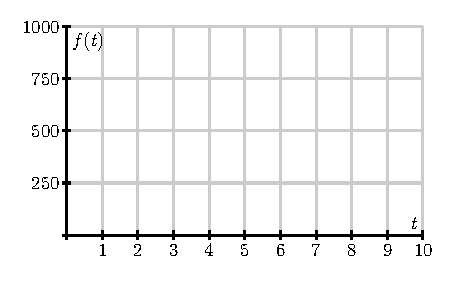
\includegraphics{figures/fig_10_2_preview_1.eps}
        \hspace*{20pt}
        \includegraphics{figures/fig_10_2_preview_2.eps}
        \caption{The graphs of $f(t)= M(0.03, t)$ and $g(r) = M(r,4)$.}
        \label{F:10.2.preview.1}
      \end{center}
    \end{figure}

  \item Find the instantaneous rate of change $f'(4)$ and state the units on
    this quantity.  What information does $f'(4)$ tell us about our
    car loan?  What information does $f'(4)$ tell us about the graph
    you sketched in (b)? 

  \item Express $M$ as a function of $r$ alone, using a fixed time of $t=4$.  That is, let $g(r) = M(r, 4)$. Sketch the graph of $g$ on the right of
    Figure \ref{F:10.2.preview.1}.  Explain the meaning of the function $g$.

  \item Find the instantaneous rate of change $g'(0.03)$ and state the units on
    this quantity.  What information does $g'(0.03)$ tell us about our
    car loan?  What information does $g'(0.03)$ tell us about the graph
    you sketched in (d)? 

    \ea


\end{pa} 

\begin{activitySolution}
 \ba
  \item If the interest rate is $r=3\% = 0.03$, and we pay the loan off in $t=4$ years, then the monthly payment is
  \[M(0.03,4) =   \frac{1500(0.03)}{1-\left(1+\frac{0.03}{12}\right)^{-12(4)}} \approx 398.42.\]

  \item If $r$ is fixed at $r=0.03$, then $M$ is a function of $t$ alone and 
\[f(t) = M(0.03,t) =  \frac{1500(0.03)}{1-\left(1+\frac{0.03}{12}\right)^{-12t}} = \frac{45}{1-1.0025^{-12t}}.\]
. The function $f$ tells us the monthly payment on a loan at different durations of time if the interest rate is fixed at $3\%$. 

  \item Using techniques from single variable calculus we have 
\[f'(t) = -\frac{(45)(12)1.0025^{-12t}\ln(1.00025)}{\left(1-1.0025^{-12t}\right)^2}.\]
So 
\[f'(4) \approx -84.54 \ \frac{\text{dollars}}{\text{year}},\]
which tells us that if we keep the interest rate constant at $3\%$, for every one year increase in the duration of the loan from 4 years there is an approximate decrease in the monthly payment of approximately 84.54 dollars. The quantity $f'(4)$ also tells us the slope of the line tangent to the graph of $f$ at $t=4$. 

  \item If $t$ is fixed at $t=4$, then $M$ is a function of $r$ alone and 
\[g(r) = M(r,4) = \frac{1500r}{1-\left(1+\frac{r}{12}\right)^{-12(4)}} = \frac{1500r}{1-\left(1+\frac{r}{12}\right)^{-48}}.\]
. The function $g$ tells us the monthly payment on a loan at different interest rates if the duration of the loan is fixed at 4 years.


  \item Using techniques from single variable calculus we have 
\[g'(r) = \frac{1500\left(1-\left(1+\frac{r}{12}\right)^{-48}\right) - 1500r\left(-48\left(1+\frac{r}{12}\right)^{-49}\right)\left(\frac{1}{12}\right)}{\left(1-\left(1+\frac{r}{12}\right)^{-48}\right)^2}.\]
So 
\[g'(0.03) \approx 795.54 \ \frac{\text{dollars}}{\text{\%}},\]
which tells us that if we keep the duration of the loan constant at 4 years, if we increase the interest rate by 1 from a rate of 3\%, the monthly payment on the loan increases by approximately \$795.54. The quantity $g'(0.03)$ also tells us the slope of the line tangent to the graph of $g$ at $r=0.03$. 

    \ea
  

\end{activitySolution}
\afterpa 

\subsection*{First-Order Partial Derivatives}

In Section \ref{S:9.1.Functions}, we studied the behavior
of a function of two or more variables by considering the {\em traces}
of the function.  Recall that in one example, we considered the function
$$
f(x,y) = \frac{x^2 \sin(2 y)}{32},
$$
which measures the range, or horizontal distance, in feet, traveled by a
projectile launched with an initial 
speed of $x$ feet per second at an angle $y$ radians to the
horizontal.  The graph of this function is given again on the left in Figure
\ref{F:10.2.trace.y}.  Moreover, if we fix the angle $y = 0.6$, we may view the trace $f(x,0.6)$ as a
function of $x$ alone, as seen at right in Figure \ref{F:10.2.trace.y}.  

%\begin{figure}[ht]
 % \begin{center}
  %      \scalebox{1.0}{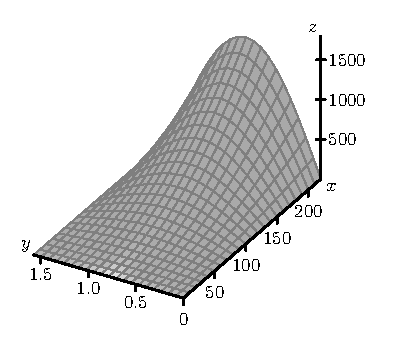
\includegraphics{figures/fig_9_1_range.eps}}
  %  \caption{The graph of $f(x,y) = x^2\sin(2y)/32$.}
 %   \label{F:10.2.range}
 % \end{center}
%\end{figure}

\begin{figure}[ht]
  \begin{center}
    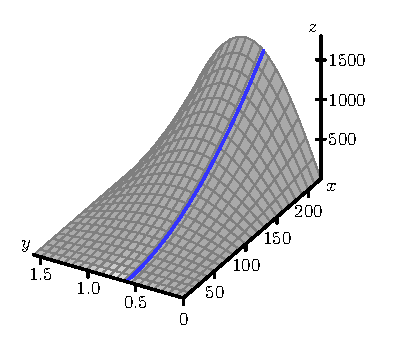
\includegraphics{figures/fig_10_2_trace_y_a.eps}
    \hspace*{0.5in}
    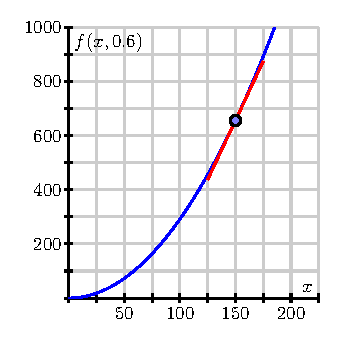
\includegraphics{figures/fig_10_2_trace_y.eps}
  \end{center}
  \caption{The trace with $y = 0.6$.}
  \label{F:10.2.trace.y}
\end{figure}

Since the trace is a one-variable function, we may consider its
derivative just as we did in the first semester of calculus.  With
$y=0.6$, we have
$$
f(x,0.6) = \frac{\sin(1.2)}{32}x^2,
$$
and therefore
$$
\frac{d}{dx}[f(x,0.6)] = \frac{\sin(1.2)}{16}x.
$$
When $x=150$, this gives
$$
\frac{d}{dx}[f(x,0.6)]|_{x=150} = \frac{\sin(1.2)}{16}150 \approx
8.74~\mbox{feet per feet per second},
$$
which gives the slope of the tangent line shown on the right of Figure 
\ref{F:10.2.trace.y}.  Thinking of this derivative as an instantaneous
rate of change implies that if we increase the initial speed of the projectile by
one foot per second, we expect the horizontal distance traveled to
increase by approximately 8.74 feet if we hold the launch angle constant at $0.6$ radians. 

By holding $y$ fixed and differentiating with respect to $x$, we
obtain the first-order {\em partial derivative of $f$ with respect to
  $x$}.  Denoting this partial derivative as $f_x$, we have seen that
$$
f_x(150, 0.6) = \frac{d}{dx}f(x,0.6)|_{x=150} = \lim_{h\to
  0}\frac{f(150+h, 0.6) - f(150, 0.6)}{h}.
$$
More generally, we have 
$$
f_x(a,b) = \lim_{h\to0} \frac{f(a+h, b)-f(a,b)}{h},
$$
provided this limit exists.

In the same way, we may obtain a trace by setting, say, $x=150$ as shown
in Figure \ref{F:10.2.trace.x}.
\begin{figure}[ht]
  \begin{center}
    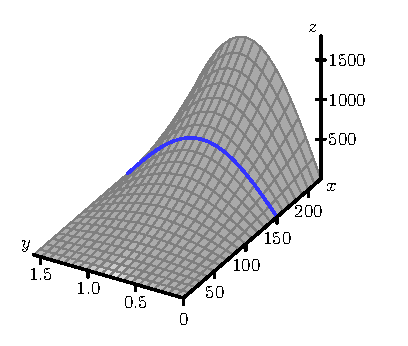
\includegraphics{figures/fig_10_2_trace_x_a.eps}
    \hspace*{0.5in}
    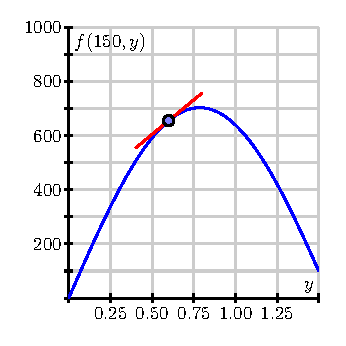
\includegraphics{figures/fig_10_2_trace_x.eps}
  \end{center}
  \caption{The trace with $x = 150$.}
  \label{F:10.2.trace.x}
\end{figure}
This gives
$$
f(150, y) = \frac{150^2}{32}\sin(2y),
$$
and therefore
$$
\frac{d}{dy}[f(150,y)] = \frac{150^2}{16}\cos(2y).
$$
If we evaluate this quantity at $y=0.6$, we have
$$
\frac{d}{dy}[f(150,y)]|_{y=0.6} = \frac{150^2}{16}\cos(1.2) \approx 509.5
~\mbox{feet per radian}.
$$
Once again, the derivative gives the slope of the tangent line shown
on the right in Figure \ref{F:10.2.trace.x}.  Thinking of the
derivative as an instantaneous rate of change, we expect that the
range of the projectile increases by 509.5 feet for every radian we increase the launch angle
$y$ if we keep the initial speed of the projectile constant at 150 feet per second.  

By holding $x$ fixed and differentiating with respect to $y$, we
obtain the first-order {\em partial derivative of $f$ with respect to $y$}.  
As before, we denote this partial derivative as $f_y$ and write
$$
f_y(150, 0.6) = \frac{d}{dy}f(150,y)|_{y=0.6} = \lim_{h\to
  0}\frac{f(150, 0.6+h) - f(150, 0.6)}{h}.
$$
As with the partial derivative with respect to $x$, we may express this quantity more generally at an arbitrary point $(a,b)$. 
To recap, we have now arrived at the formal definition of the first-order partial derivatives of a function of two variables.

\vspace*{5pt}
\nin \framebox{\hspace*{3 pt}
  \parbox{6.25 in}{ \begin{definition} The first-order \textbf{partial
        derivatives of $f$ with respect to $x$ and $y$}\index{partial
        derivatives!first-order} at a point $(a,b)$ are, respectively,
    \begin{align*}
      f_x(a,b) & = \lim_{h \to 0} \frac{f(a+h,b)-f(a,b)}{h}, \ \mbox{and} \\
      f_y(a,b) & = \lim_{h \to 0} \frac{f(a,b+h)-f(a,b)}{h}, \\
    \end{align*}
    provided the limits exist.
\end{definition}
} \hspace*{3 pt}}
\vspace*{5pt}

 \begin{activity} \label{A:10.2.10} Consider the function $f$ defined by 
   $$
   f(x,y) = \frac{xy^2}{x+1}
   $$
   at the point $(1,2)$.

   \ba
   \item Write the trace $f(x,2)$ at the fixed value $y=2$.   
     On the left side of Figure \ref{F:10.2.activity.trace},
     draw the graph of the trace with $y=2$ indicating the scale and
     labels on the axes.  Also, sketch 
     the tangent line at the point $x=1$.

   \begin{figure}[ht]
     \begin{center}
       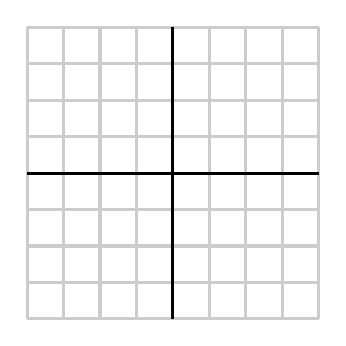
\includegraphics{figures/fig_10_2_empty.eps}
       \hspace*{0.5in}
       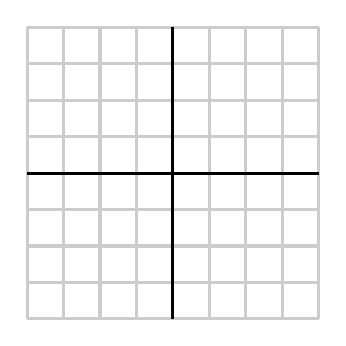
\includegraphics{figures/fig_10_2_empty.eps}
     \end{center}
     \caption{Traces of $f(x,y) = \frac{xy^2}{x+1}$.}
     \label{F:10.2.activity.trace}
   \end{figure}

   \item Find the partial derivative $f_x(1,2)$ and relate its value
     to the sketch you just made.

   \item Write the trace $f(1,y)$ at the fixed value $x=1$.  
     On the right side of Figure \ref{F:10.2.activity.trace},
     draw the graph of the trace with $x=1$ indicating the scale and
     labels on the axes.  Also, sketch 
     the tangent line at the point $y=2$.

   \item Find the partial derivative $f_y(1,2)$ and relate its value
     to the sketch you just made.


   \ea


\end{activity}

\begin{activitySolution}
\ba
\item Here we have $f(x,2) = \frac{4x}{x+1}$. At the point where $x=1$, the tangent line to this trace has slope $\frac{d}{dx} f(x,2) \left. \right|_{x=1} = 1$, and so the line tangent to the graph of this trace at $x=1$ has equation $z=2+(x-1)$. 
\item Now $f_x(x,y) = \frac{(x+1)(y^2) - xy^2}{(x+1)^2}$, and so $f_x(1,2) = \frac{8-4}{4} = 1$. This is the slope of the line tangent to the trace $f(x,2)$ at the point where $x=1$, as calculated in part (a). 
\item Here we have $f(1,y) = \frac{1}{2}y^2$. At the point where $y=2$, the tangent line to this trace has slope $\frac{d}{dy} f(1,y) \left. \right|_{y=2} = 2$, and so the line tangent to the graph of this trace at $y=2$ has equation $z=2+2(y-2)$. 
\item Now $f_y(x,y) = \frac{x}{x+1}(2y)$, and so $f_y(1,2) = 2$. This is the slope of the line tangent to the trace $f(1,y)$ at the point where $y=2$, as calculated in part (c).  
\ea
\end{activitySolution}

\aftera


As these examples show, each partial derivative at a point arises as
the derivative of a one-variable function defined by fixing one of the
coordinates.  In addition, we may consider each partial derivative as defining a new
function of the point $(x,y)$, just as the derivative $f'(x)$ defines
a new function of $x$ in single-variable calculus.  Due to the connection between one-variable
derivatives and partial derivatives, we will often use Leibniz-style
notation to denote partial derivatives by writing
$$
\frac{\partial f}{\partial x}(a, b) = f_x(a,b),
\hspace*{20pt}
\mbox{and}
\hspace*{20pt}
\frac{\partial f}{\partial y}(a, b) = f_y(a,b).
$$

To calculate the partial
derivative $f_x$, we hold $y$ fixed and thus we treat $y$ as a
constant.  In Leibniz notation, observe that 
$$
\frac{\partial }{\partial x} (x) = 1
\hspace*{20pt}
\mbox{and}
\hspace*{20pt}
\frac{\partial }{\partial x}(y) = 0.
$$
To see the contrast between how we calculate single variable derivatives and partial derivatives, and the difference between the notations $\frac{d}{dx}[ \ ]$ and $\frac{\partial}{\partial x}[ \ ]$, observe that
\begin{align*}
  & \frac{d}{dx}[3x^2 - 2x + 3] = 3\frac{d}{dx}[x^2] - 2\frac{d}{dx}[x]
  + \frac{d}{dx}[3] = 3\cdot 2x - 2, \\
  \mbox{and}\hspace*{20pt} & \frac{\partial}{\partial x}[x^2y - xy + 2y] =
  y\frac{\partial}{\partial x}[x^2] -
  y\frac{\partial}{\partial x}[x]
  + \frac{\partial}{\partial x}[2y] = y\cdot 2x - y 
\end{align*}
Thus, computing partial derivatives is straightforward:  we use the standard rules of single variable calculus, but do so while holding one (or more) of the variables constant.

\begin{activity} \label{A:10.2.2} 
  \ba
\item If we have the function $f$ of the variables $x$ and $y$ and we want to find the partial derivative
  $f_x$, which variable do we treat as a constant?  When we find the
  partial derivative $f_y$, which variable do we treat as a constant?

\item If $f(x,y) = 3x^3 - 2x^2y^5$, find the partial derivatives $f_x$
  and $f_y$.

\item If $f(x,y) = \displaystyle\frac{xy^2}{x+1}$, find the partial
  derivatives $f_x$ and $f_y$.

\item If $g(r,s) = rs\cos(r)$, find the partial derivatives $g_r$ and
  $g_s$. 
		
\item Assuming $f(w,x,y) = (6w+1)\cos(3x^2+4xy^3+y)$, find the partial
  derivatives $f_w$, $f_x$, and $f_y$.
	
\item Find all possible first-order partial derivatives of $q(x,t,z) =
  \displaystyle \frac{x2^tz^3}{1+x^2}.$
	
  \ea

\end{activity}
\begin{smallhint}

\end{smallhint}
\begin{bighint}

\end{bighint}
\begin{activitySolution}
	\ba
	\item When we differentiate with respect to $x$, we treat $y$ as a constant. So the power and scalar multiple rules give us
\[\frac{\partial f}{\partial x} = 9x^2 - 4y^5x.\]
Similarly,
\[\frac{\partial f}{\partial y} = -10x^2y^4.\]
		
	
	\item When we differentiate with respect to $r$, we treat $s$ as a constant. So the product rule give us 
\[g_r(r,s) = -rs\sin(r) + s\cos(r).\]
Using the scalar multiple rule we have
\[g_s(r,s) = r\cos(r).\]
		
	\item When we differentiate with respect to $w$, we treat $x$ and $y$ as constants. So the scalar multiple rule give us 
\[\frac{\partial f}{\partial w} = 6\cos(3x^2+4xy^3+y).\]
To differentiate with respect to $x$ will require the scalar multiple and chain rules, giving us
\[\frac{\partial f}{\partial x} = -(6w+1)\sin(3x^2+4xy^3+y)(6x+4y^3).\]
Similarly,
\[\frac{\partial f}{\partial y} = -(6w+1)\sin(3x^2+4xy^3+y)(12xy^2+1).\]	
		
	\item When we differentiate with respect to $x$, we treat $t$ and $z$ as constants. So the scalar multiple and quotient rules give us 
\[q_x(x,t,z) = \frac{(1+x^2)(2^tz^3)-(x2^tz^3)(2x)}{(1+x^2)^2}.\]
To differentiate with respect to $t$, we hold $x$ and $z$ constant to obtain
\[q_t(x,t,z) = \frac{1}{1+x^2}(x2^t\ln(2)z^3)\]
and
\[q_z(x,t,z) = \frac{1}{1+x^2}(3x2^tz^2).\]
		
	\ea

\end{activitySolution}
\aftera


\subsection*{Interpretations of First-Order Partial Derivatives}

Recall that the derivative of a single variable function has a
geometric interpretation as the slope of the line tangent to the graph
at a given point.  Similarly, we have seen that the partial
derivatives measure the slope of a line tangent to a trace of a
function of two variables as shown in Figure
\ref{F:10.2.trace.tangent}. 

\begin{figure}[ht]
  \begin{center}
    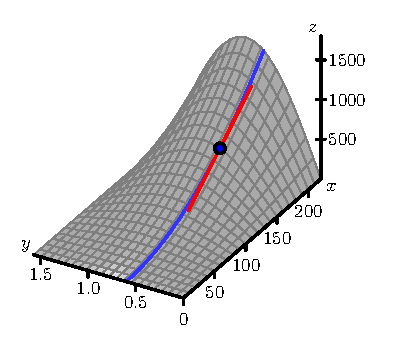
\includegraphics{figures/fig_10_2_trace_tangent_y.eps}
    \hspace*{0.5in}
    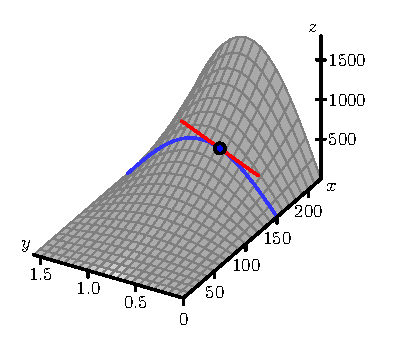
\includegraphics{figures/fig_10_2_trace_tangent_x.eps}
  \end{center}
  \caption{Tangent lines to two traces of the range function.} 
  \label{F:10.2.trace.tangent}
\end{figure}

Now we consider the first-order partial derivatives in context. Recall
that the difference quotient $\frac{f(a+h)-f(a)}{h}$ for a function
$f$ of a single variable $x$ at a point where $x=a$ tells us the
average rate of change of $f$ over the interval $[a,a+h]$, while the
derivative $f'(a)$ tells us the instantaneous rate of change of $f$ at
$x=a$.
We can use these same concepts to
explain the meanings of the partial derivatives in context.

\begin{activity} \label{A:10.2.11} 
The speed of sound $C$ traveling through ocean water is a function of
temperature, salinity and depth.  It may be modeled by the function
$$
C=1449.2+4.6T-0.055T^2+0.00029T^3+(1.34-0.01T)(S-35)+0.016D.
$$
Here $C$ is the speed of sound in meters/second, $T$ is the
temperature in degrees Celsius, $S$ is the salinity in grams/liter of
water, and $D$ is the depth below the ocean surface in meters.

\ba
\item State the units in which each of the partial derivatives,
  $C_T$, $C_S$ and $C_D$, are expressed and explain the physical
  meaning of each. 

\item Find the partial derivatives $C_T$, $C_S$ and $C_D$.  

\item Evaluate each of the three partial derivatives at the point where $T=10$, $S=35$ and
  $D=100$.  What does the sign of each partial derivatives tell us about the behavior of the function $C$ at the point $(10,35, 100)$?

  \ea


\end{activity}

\begin{activitySolution}
\ba
\item The partial derivative $C_T$ is defined in terms of a change in $C$ per change in $T$. So the units of $C_T$ are units of $C$ over units of $T$, or $\frac{\frac{\text{m}}{\text{sec}}}{^{\circ}C}$. This partial $C_T$ approximates how the speed of sound changes for every degree Celsius increase in the temperature of the water.

Similarly, the units of $C_S$ are $\frac{\frac{\text{m}}{\text{sec}}}{\frac{g}{l}}$. This partial $C_S$ approximates how the speed of sound changes for every gram per liter increase of the salinity of the water.

Finally, the units of $C_D$ are $\frac{\frac{\text{m}}{\text{sec}}}{m}$. This partial $C_D$ approximates how the speed of sound changes for every meter increase in depth below the ocean surface. 
\item Here we have 
\begin{align*}
C_T &= 4.6-0.11T+0.00087T^2-0.01(S-35) \\
C_S &= 1.34-0.01T \\
C_D &= 0.016.
\end{align*}
\item Evaluating the partial derivatives at the point (10,35,100) gives us 
\begin{align*}
C_T(10,35,100) &= 3.587 \\
C_S(10,35,100) &= 1.24 \\
C_D(10,35,100) &= 0.016.
\end{align*}
That $C_T(10,35,100)$ is positive tells us that if we increase the temperature from $10^{\circ}C$ while holding the salinity constant at 35 grams per liter and the depth constant at 100 meters, the speed of sound in the ocean increases. Similarly, the fact that $C_S(10,35,100)$ is positive tells us that if we increase salinity from 35 grams per liter while holding the the temperature constant at $10^{\circ}C$ and the depth constant at 100 meters, the speed of sound in the ocean increases. Also, the fact that $C_D(10,35,100)$ is positive tells us that if we increase depth from 100 meters while holding the the temperature constant at $10^{\circ}C$ and the salinity constant at 35 grams per liter, the speed of sound in the ocean increases. 
\ea
\end{activitySolution}

\aftera


\subsection*{Using tables and contours to estimate partial
  derivatives} 

Remember that functions of two variables are often represented as either
a table of data or a contour plot.
In single variable calculus, we saw how we can use the difference
quotient to approximate derivatives if, instead of an algebraic
formula, we only know the value of the
function at a few points.
The same idea applies to partial derivatives.

\begin{activity} \label{A:10.2.12} The wind chill, as frequently
  reported, is a measure of how cold it feels outside when
  the wind is blowing.  In Table \ref{T:10.2.wind.chill}, the wind
  chill $w$, measured in degrees Fahrenheit, is a function of the wind speed $v$, measured in miles per hour, and
  the ambient air temperature $T$, also measured in degrees
  Fahrenheit.  We thus view $w$ as being of the form $w = w(v, T)$.

\begin{table}[ht] 
  \begin{center}
    \begin{tabular}{|c||c|c|c|c|c|c|c|c|c|c|c|}
      \hline
      $v \backslash T$  
         &-30  &-25 &-20 &-15 &-10 &-5  &0   &5   &10  &15  &20  \\
      \hhline{|=|=|=|=|=|=|=|=|=|=|=|=|}
      5  &-46	&-40 &-34 &-28 &-22 &-16 &-11 &-5 &1 &7 &13  \\
      \hline
      10 &-53	&-47 &-41 &-35 &-28 &-22 &-16 &-10 &-4 &3 &9   \\
      \hline
      15 &-58	&-51 &-45 &-39 &-32 &-26 &-19 &-13 &-7 &0 &6  \\
      \hline
      20 &-61	&-55 &-48 &-42 &-35 &-29 &-22 &-15 &-9 &-2 &4  \\
      \hline
      25 &-64	&-58 &-51 &-44 &-37 &-31 &-24 &-17 &-11 &-4 &3 \\
      \hline
      30 &-67	&-60 &-53 &-46 &-39 &-33 &-26 &-19 &-12 &-5 &1 \\
      \hline
      35 &-69	&-62 &-55 &-48 &-41 &-34 &-27 &-21 &-14 &-7 &0 \\
      \hline
      40 &-71	&-64 &-57 &-50 &-43 &-36 &-29 &-22 &-15 &-8 &-1 \\
      \hline
    \end{tabular}
    \caption{Wind chill as a function of wind speed and temperature.}
    \label{T:10.2.wind.chill}
  \end{center}
\end{table}
%\begin{table}[ht]
%  \begin{center}
%    \begin{tabular}{|c||c|c|c|c|c|c|c|c|c|c|c|}
%      \hline
%      $v \backslash T$  
%         &-30  &-25 &-20 &-15 &-10 &-5  &0   &5   &10  &15  &20  \\
%      \hhline{|=|=|=|=|=|=|=|=|=|=|=|=|}
%      5  &-35  &-31 &-26 &-20 &-15 &-11 &-6  &1   &7   &12  &16  \\
%      \hline
%      10 &-58  &-52 &-45 &-38 &-31 &-27 &-22 &-15 &-9  &-2  &2   \\
%      \hline
%      15 &-70  &-65 &-60 &-51 &-45 &-40 &-33 &-25 &-18 &-11 &-6  \\
%      \hline
%      20 &-81  &-76 &-68 &-60 &-52 &-46 &-40 &-32 &-24 &-17 &-9  \\
%      \hline
%      25 &-89  &-83 &-75 &-67 &-58 &-52 &-45 &-37 &-29 &-22 &-15 \\
%      \hline
%      30 &-94  &-87 &-78 &-70 &-63 &-56 &-49 &-41 &-33 &-26 &-18 \\
%      \hline
%      35 &-98  &-90 &-83 &-72 &-67 &-60 &-52 &-43 &-35 &-27 &-20 \\
%      \hline
%      40 &-101 &-94 &-87 &-76 &-69 &-62 &-54 &-45 &-36 &-29 &-22 \\
%      \hline
%    \end{tabular}
%    \caption{Wind chill as a function of temperature and wind speed}
%    \label{T:10.2.wind.chill}
%  \end{center}
%\end{table}

\ba
\item Estimate the partial derivative $w_v(20,-10)$.  What are the
  units on this quantity and what does it mean?
\item Estimate the partial derivative $w_T(20,-10)$.  What are the
  units on this quantity and what does it mean?
\item Use your results to estimate the wind chill $w(18, -10)$.
\item Use your results to estimate the wind chill $w(20, -12)$.
\item Use your results to estimate the wind chill $w(18, -12)$.
\ea

\end{activity}

\begin{activitySolution}
\ba
\item Recall that 
\[w_v(v,T) = \lim_{h \to 0} \frac{w(v+h,T) - w(v,T)}{h},\]
which gives us the slope of the tangent line to the trace in the $v$ direction. We can approximate this slope with the slope of a secant line, choosing points equally spaced on both sides of $(v,T)$. In other words,
\[w_v(v,T) \approx \frac{w(v+h,T) - w(v-h,T)}{2h},\]
for small values of $h$. This is the symmetric difference quotient from calculus 1. 
The data in our table allows us to use $h=5$ for wind speed, so 
\[w_v(20,-10) \approx \frac{w(25,-10)-w(15,-10)}{10} = \frac{-37-(-32)}{10} = -\frac{1}{2}\]
degrees Fahrenheit per mile per hour. So for every one mile per hour increase in the wind speed from 20 miles per hour, while holding the air temperature constant at $-10^{\circ}F$, the wind chill decreases by approximately 0.5 $^{\circ}F$. 
\item We approximate $w_T(20,-10)$ in the same way, using $h=5$ again. So 
\[w_T(20,-10) \approx \frac{w(20,-5)-w(20,-15)}{10} = \frac{-29-(-42)}{10} = 1.3\]
degrees Fahrenheit per degree Fahrenheit. So for every one degree Fahrenheit increase in the wind temperature $-10^{\circ}F$, while holding the wind speed constant at 20 miles per hour, the wind chill increases by approximately 1.3 $^{\circ}F$.  
\item This is just like a linearization from calculus 1 along the trace with $T=-10$. We found the slope of the tangent line to the $T=-10$ trace of $w$ at the point $(20,-10)$ to be $-0.5$, so  
\[w(18,-10) \approx  w(20,-10) - 0.5(18-20) = -35 + 1 = -34.\]
\item This is just like a linearization from calculus 1 along the trace with $v=20$. We found the slope of the tangent line to the $v=20$ trace of $w$ at the point $(20,-10)$ to be $1.3$, so  
\[w(20,-12) \approx  w(20,-10) + 1.3(-12-(-10)) = -35 - 2.6 = -37.6.\]
\item We might expect that the total change in $w$ will be calculated by using the changes in $w$ that arise from changing both the $v$ and $T$ coordinates. In other words,
\[w(18,-12) \approx w(20,-10) - 0.5(18-20) + 1.3(-12-(-10)) = -35 + 1 - 2.6 = -36.6.\]
\ea
\end{activitySolution}

\aftera


\begin{activity} \label{A:10.2.13} 
  Shown below in Figure \ref{F:10.2.activity.contour} is a contour
  plot of a function $f$.  The value of the function along a few
  of the contours is indicated to the left of the figure.

\begin{figure}[ht]
  \begin{center}
    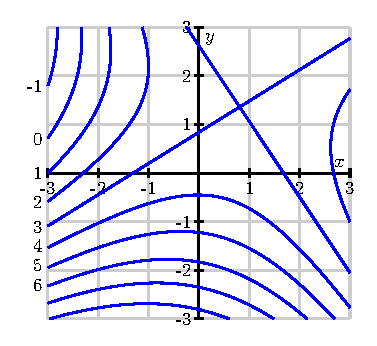
\includegraphics{figures/fig_10_2_activity_contours.eps}
    \caption{A contour plot of $f$.}
    \label{F:10.2.activity.contour}
  \end{center}
\end{figure}

\ba
\item Estimate the partial derivative $f_x(-2,-1)$.  
\item Estimate the partial derivative $f_y(-2,-1)$.
\item Estimate the partial derivatives $f_x(-1,2)$ and $f_y(-1,2)$.  
\item Locate one point $(x,y)$ where the partial derivative $f_x(x,y)=
  0$. 
\item Locate one point $(x,y)$ where $f_x(x,y)<0$.
\item Locate one point $(x,y)$ where $f_y(x,y)>0$.
\item Suppose you have a different function $g$, and you know that $g(2,2) =
  4$, $g_x(2,2) > 0$, and $g_y(2,2) > 0$.  Using this information,
  sketch a possibility for the contour $g(x,y)=4$ passing through
  $(2,2)$ on the left side of Figure \ref{F:10.2.activity.grad}.  Then
  include possible contours $g(x,y) = 3$ and $g(x,y) = 5$.

  \begin{figure}[ht]
    \begin{center}
      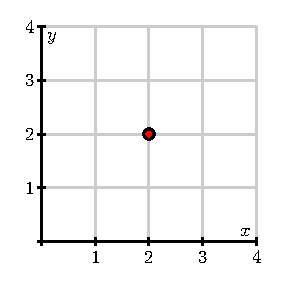
\includegraphics{figures/fig_10_2_activity_grad.eps}
      \hspace*{1in}
      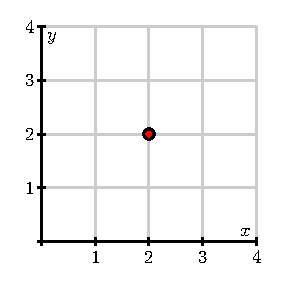
\includegraphics{figures/fig_10_2_activity_grad.eps}
    \end{center}
    \caption{Plots for contours of $g$ and $h$.}
    \label{F:10.2.activity.grad}
  \end{figure}
\item Suppose you have yet another function $h$, and you know that $h(2,2) =
  4$, $h_x(2,2) < 0$, and $h_y(2,2) > 0$.  Using this information,
  sketch a possible contour $h(x,y)=4$ passing through
  $(2,2)$ on the right side of Figure \ref{F:10.2.activity.grad}.
  Then include possible contours $h(x,y) = 3$ and $h(x,y) = 5$.
    
\ea

\end{activity}

\begin{activitySolution}
\ba
\item Recall that 
\[f_x(x,y) = \lim_{h \to 0} \frac{f(x+h,y) - f(x,y)}{h},\]
which gives us the slope of the tangent line to the trace in the $x$ direction. We can approximate this slope with the slope of a secant line, choosing points equally spaced on both sides of $(x,y)$. In other words,
\[f_x(x,y) \approx \frac{f(x+h,y) - f(x-h,y)}{2h},\]
for small values of $h$. This is the symmetric difference quotient from calculus 1. 
Using $h=1$ and approximating values from the contour plot gives us  
\[f_x(-2, -1) \approx \frac{f(-1,-1)-f(-3,-1)}{2} \approx \frac{4.5-2.9}{2} = 0.8.\] 
\item We approximate $f_y(-2,-1)$ in the same way, using $h=1$ again. So 
\[f_y(-2,-1) \approx \frac{f(-2,0)-f(-2,-2)}{2} \approx \frac{2.4-6}{2} = -1.8.\]
\item As above, 
\begin{align*}
f_x(-1,2) &\approx \frac{f(0,2)-f(-2,2)}{2} \approx \frac{3-0.8}{2} = 1.1 \\
f_y(-1,2) &\approx \frac{f(-1,3)-f(-1,1)}{2} \approx \frac{2.1-2.3}{2} = -0.1.
\end{align*}
\item A point at which $f_x(x,y) = 0$ will occur when we have a horizontal tangent line. Such a point occurs near $(0,-0.5)$. 
\item A point at which $f_y(x,y) = 0$ will occur when we have a vertical tangent line. Such a point occurs near $(-1,2)$. 
\item We want a point at which $f$ is decreasing in the $x$-direction. Such a point is $(2,-2)$.
\item We want a point at which $f$ is increasing in the $y$-direction. Such a point is $(-1.2,-1)$.
\item A possible plot is shown at left below.
\item A possible plot is shown at right below.
    \begin{center}
      \resizebox{!}{2.0in}{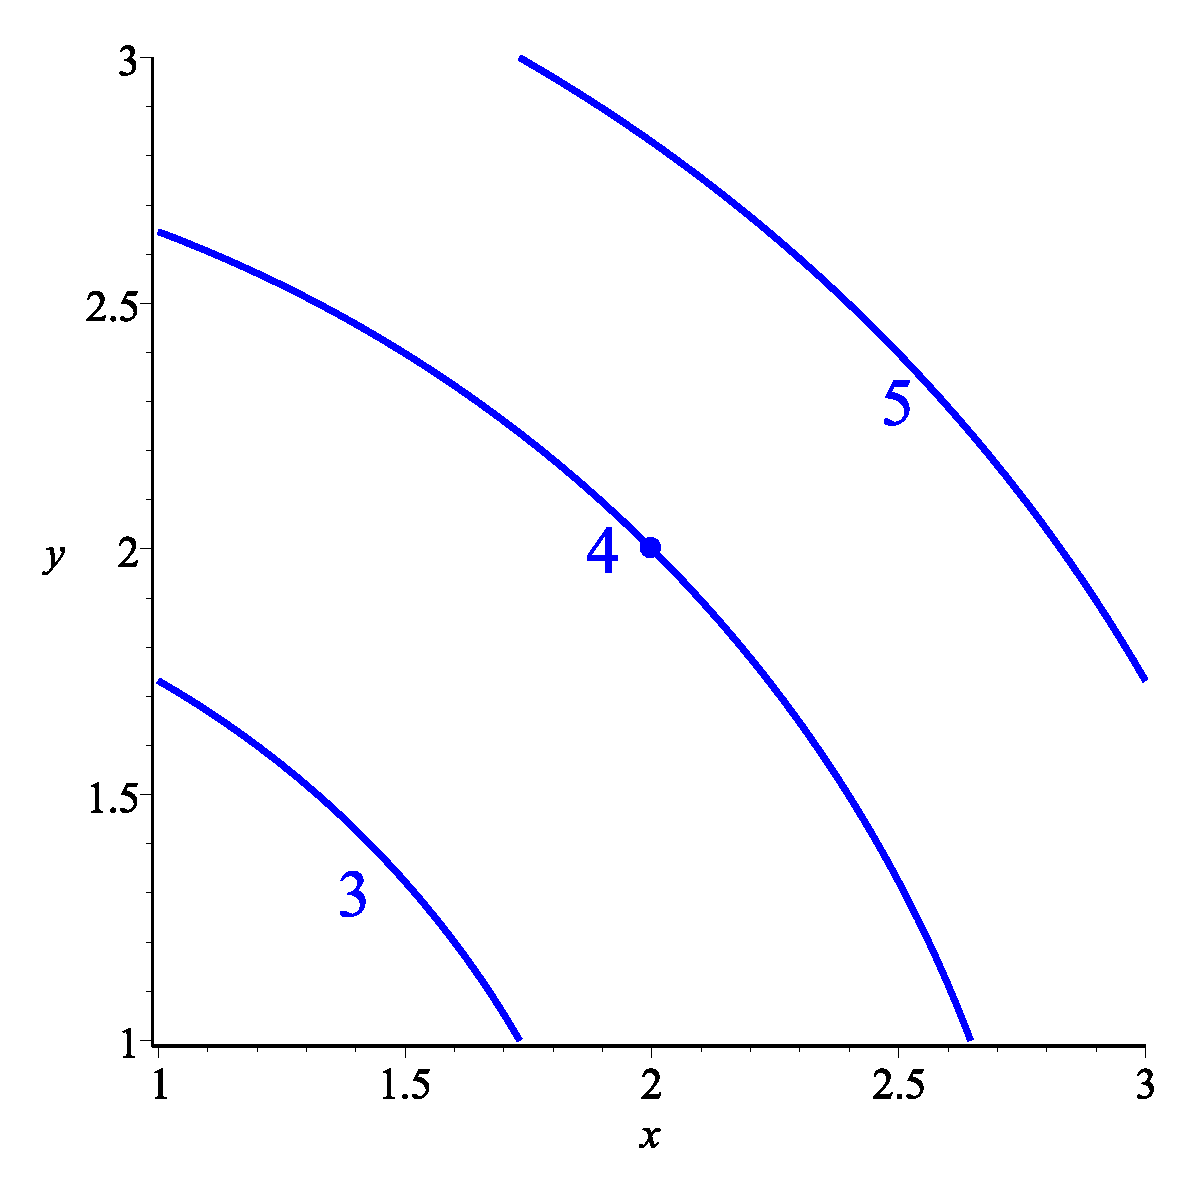
\includegraphics{figures/fig_10_2_activity_grad_g.eps}}
      \hspace*{1in}
      \resizebox{!}{2.0in}{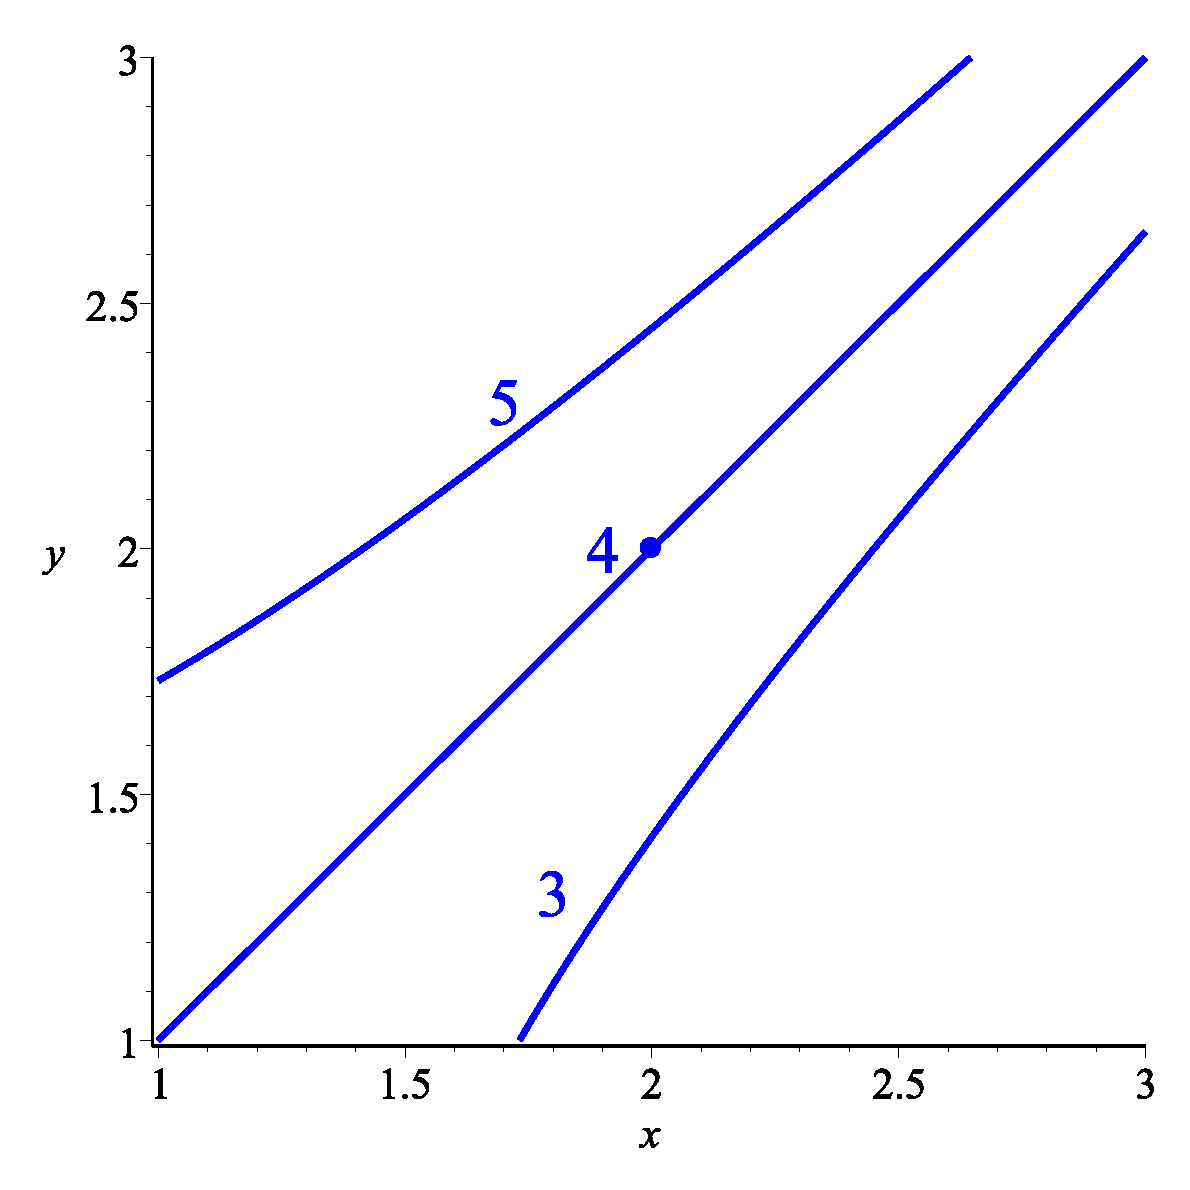
\includegraphics{figures/fig_10_2_activity_grad_h.eps}}
    \end{center}
\ea
\end{activitySolution}


\aftera


\begin{summary}
\item If $f(x,y)$ is a function of two variables, there are two first
  order partial derivatives of $f$: the partial derivative of $f$ with respect to $x$,
      \[\frac{\partial f}{\partial x}(x,y) = f_x(x,y) = \lim_{h \to 0}
      \frac{f(x+h,y) - f(x,y)}{h},\]
      and the partial derivative of $f$ with respect to $y$,
      \[\frac{\partial f}{\partial y}(x,y) = f_y(x,y) = \lim_{h \to 0}
      \frac{f(x,y+h) - f(x,y)}{h},\] 
      where each partial derivative exists only at those points $(x,y)$ for which
      the limit exists.
  \item The partial derivative $f_x(a,b)$ tells us the instantaneous rate of
    change of $f$ with respect to $x$ at $(x,y) = (a,b)$ when $y$ is fixed at $b$.  Geometrically,
    the partial derivative $f_x(a,b)$ tells us the slope of the line
    tangent to the $y=b$ trace of the function $f$ at the point
    $(a,b,f(a,b))$.
  \item The partial derivative $f_y(a,b)$ tells us the instantaneous rate of
    change of $f$ with respect to $y$ at $(x,y) = (a,b)$ when $x$ is fixed at $a$.  Geometrically,
    the partial derivative $f_y(a,b)$ tells us the slope of the line
    tangent to the $x=a$ trace of the function $f$ at the point
    $(a,b,f(a,b))$.
\end{summary}


\nin \hrulefill

%\newpage
\begin{exercises} 

\item \label{Ez:10.2.1}   The Heat Index, $I$, (measured in \emph{apparent degrees F}) is a function of the actual temperature $T$ outside (in degrees F) and the relative humidity $H$ (measured as a percentage).  A portion of the table which gives values for this function, $I(T,H)$, is reproduced below:
\begin{center}
\begin{tabular}{|l||r|r|r|r|} \hline
\emph{T} $\downarrow \backslash$ \emph{H} $\rightarrow$ 
	& 70 &	75 & 80 &	85  \\ \hhline{|=|=|=|=|=|}
90 & 106 & 109 & 112 & 115  \\ \hline
92 & 112 & 115 & 119 & 123  \\ \hline
94 & 118 & 122 & 127 & 132  \\ \hline
96 & 125 & 130 & 135 & 141  \\ \hline
\end{tabular}
\end{center}

				
    \ba
   	\item State the limit definition of the value $I_T(94,75)$.  Then, estimate $I_T(94,75)$, and write one complete sentence that carefully explains the meaning of this value, including its units.	
	
	\item State the limit definition of the value $I_H(94,75)$.  Then, estimate $I_H(94,75)$, and write one complete sentence that carefully explains the meaning of this value, including its units.
	
	\item Suppose you are given that $I_T(92,80) = 3.75$ and $I_H(92,80) = 0.8$.  Estimate the values of $I(91,80)$ and $I(92,78)$.  Explain how the partial derivatives are relevant to your thinking.
	
	\item On a certain day, at 1 p.m. the temperature is 92 degrees and the relative humidity is 85\%.  At 3 p.m., the temperature is 96 degrees and the relative humidity 75\%.  What is the average rate of change of the heat index over this time period, and what are the units on your answer?  Write a sentence to explain your thinking.
	
%	\item (6) Recall the given information from (b) that $I_T(92,80) = 3.75$ and $I_H(92,80) = 0.8$.  Suppose that on a day when the temperature is 92$^\circ$ with relative humidity of 80\%, at the time these data are recorded, the actual temperature is decreasing at a rate of 2 degrees per hour and relative humidity is rising at a rate of 3\% per hour.  At what instantaneous rate is the heat index changing at this time?  What are the relevant units on this rate of change?  Write a sentence to clearly explain your thinking in this problem and justify your answer.
    \ea

\begin{exerciseSolution}
\ba
   	\item The limit definition of the value $I_T(94,75)$ is
\[I_T(94,75) = \lim_{h \to 0} \frac{I(94+h,75)-I(94,75}{h}.\]
We can use a symmetric difference quotient to estimate $I_T(94,75)$:
\[I_T(94,75) \approx \frac{I(94+2,75)-I(94-2,75)}{4} = \frac{13}{4} = 3.25.\]
The number $I_T(94,75)$ tells us that if the temperature increases by $1^{\circ}$F from $94^{\circ}$F while the relative humidity remains constant at 75\%, the heat index increases by approximately $3.25^{\circ}$F. In other words, it feels approximately $3.25^{\circ}$F warmer if the temperature increases by $1^{\circ}$F from $94^{\circ}$F while the relative humidity remains constant at 75\%.
	
	\item The limit definition of the value $I_H(94,75)$ is
\[I_H(94,75) = \lim_{h \to 0} \frac{I(94,75+h)-I(94,75}{h}.\]
We can use a symmetric difference quotient to estimate $I_H(94,75)$:
\[I_H(94,75) \approx \frac{I(94,75+5)-I(94,75-5)}{10} = \frac{9}{10} = 0.9.\]
The number $I_H(94,75)$ tells us that if the relative humidity increases by 1\% from 75\% while the temperature remains constant at $94^{\circ}$F, the heat index increases by approximately $0.9^{\circ}$F. In other words, it feels approximately $0.9^{\circ}$F warmer if the relative humidity increases by 1\% from 75\% while the temperature remains constant at $94^{\circ}$F, the heat index increases by approximately $0.9^{\circ}$F.
	
	\item By definition,  
\[I_T(92,80) \approx \frac{I(91,80)-I(92,80)}{-1},\]
so 
	\[I(91,80) \approx I(92,80) - I_T(92,80) = 119-3.75 = 115.25.\]
Similarly, by definition,  
\[I_T(92,80) \approx \frac{I(92,78)-I(92,80)}{-2},\]
so 
	\[I(92,78) \approx I(92,80) - 2I_H(92,80) = 119-2(0.8) = 117.4.\]

	\item The average rate of change of the heat index over this time period will be the change in the heat index divided by the time. So the average rate of change of the heat index from 1 p.m. to 3 p.m. is 
\[\frac{I(96,75)-I(92,85)}{3-1} = \frac{130-123}{2} = 3.5 \ \frac{^{\circ}\text{F}}{\text{hour}}.\]
\ea

\end{exerciseSolution}

\item \label{Ez:10.2.1.5} Let $f(x,y) = \frac{1}{2}xy^2$ represent the kinetic energy in Joules of an object of mass $x$ in kilograms with velocity $y$ in meters per second. Let $(a,b)$ be the point $(4,5)$ in the domain of $f$.
    \ba
    \item Calculate $f_x(a,b)$.
    
    \item Explain as best you can in the context of kinetic energy what the partial derivative
\[f_x(a,b) = \lim_{h \to 0} \frac{f(a+h,b) - f(a,b)}{h}\]
tells us about kinetic energy.

    \item Calculate $f_y(a,b)$.

    \item Explain as best you can in the context of kinetic energy what the partial derivative
\[f_y(a,b) = \lim_{h \to 0} \frac{f(a,b+h) - f(a,b)}{h}\]
tells us about kinetic energy.



     \item Often we are given certain graphical information about a function instead of a rule. We can use that information to approximate partial derivatives. For example, suppose that we are given a contour plot of the kinetic energy function (as in Figure \ref{F:10.2.pd_contour}) instead of a formula. Use this contour plot to approximate $f_x(4,5)$ and $f_y(4,5)$ as best you can. Compare to your calculations from earlier parts of this exercise.  
\begin{figure}[ht]
  \begin{center}
%       \scalebox{0.5}{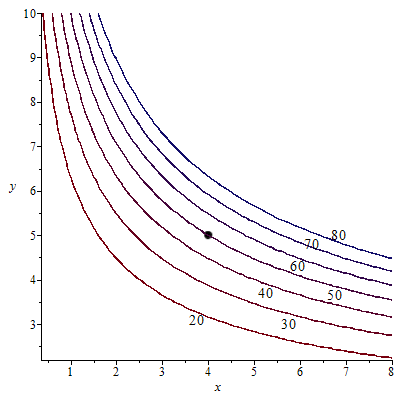
\includegraphics{figures/10_2_pd_contour}}
    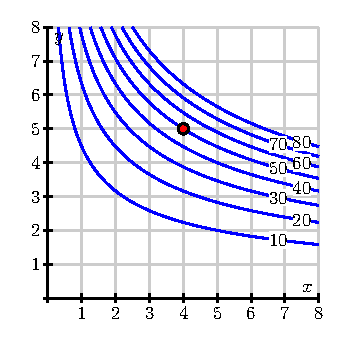
\includegraphics{figures/fig_10_2_ke_contour.eps}
    \caption{The graph of $f(x,y) = \frac{1}{2}xy^2$.}
    \label{F:10.2.pd_contour}
  \end{center}
\end{figure}
    \ea
\begin{exerciseSolution}
    \ba
    \item A straightforward calculation shows that 
\[f_x(x,y) = \frac{1}{2}y^2.\]
So 
\[f_x(a,b) = \frac{1}{2}(5^2) = 12.5.\]

    \item The value of $f_x(a,b)$ tells us that if the mass of the object increases by 1 kg from 4 kg while the velocity of the object remains constant at 5 meters per second, the kinetic energy of the object increases by approximately 12.5 Joules. 

    \item A straightforward calculation shows that 
\[f_y(x,y) = xy.\]
So 
\[f_y(a,b) = (4)(5) = 20.\]

    \item The value of $f_y(a,b)$ tells us that if the velocity of the object increases by one meter per second from a velocity of 5 meters per second while the mass remains constant at 4 kg, the kinetic energy of the object increases by approximately 20 Joules. 

		\item To approximate $f_x(4,5)$, we will use a symmetric difference quotient. That is,
\[f_x(4,5) \approx \frac{f(4+h,5)-f(4-h,5)}{2h}\]
for a suitable value of $h$. We can approximate the values of $f$ on the contour plot for $h = 1$, giving us 
\[f_x(4,5) \approx  \frac{f(5,5)-f(3,5)}{2} \approx \frac{60-40}{2} = 10.\]
Similarly,
\[f_y(4,5) \approx  \frac{f(4,6)-f(4,4)}{2} \approx \frac{65-30}{2} = 17.5.\]
These values compare reasonably well to the values of $f_x(4,5) = 12.5$ and $f_y(4,5) = 20$ obtained earlier.
    \ea

\end{exerciseSolution}

\item \label{Ez:10.2.2}    The temperature on an unevenly heated metal plate positioned in the first quadrant of the $x$-$y$ plane is given by 
$$C(x,y) = \frac{25xy+25}{(x-1)^2 + (y-1)^2 + 1}.$$
Assume that temperature is measured in degrees Celsius and that $x$ and $y$ are each measured in inches. ({\bf Note:} At no point in the following questions should you expand the denominator of $C(x,y)$.)

\ba

	\item Determine $\frac{\partial C}{\partial x}|_{(x,y)}$ and $\frac{\partial C}{\partial y}|_{(x,y)}$.  

	\item If an ant is on the metal plate, standing at the point $(2,3)$, and starts walking in a direction parallel to the $y$ axis, at what rate will the temperature he is experiencing change?  Explain, and include appropriate units.

	\item If an ant is walking along the line $y = 3$, at what instantaneous rate will the temperature he is experiencing change when he passes the point $(1,3)$?

	\item Now suppose the ant is stationed at the point $(6,3)$ and walks in a straight line towards the point $(2,0)$.  Determine the \emph{average} rate of change in temperature (per unit distance traveled) the ant encounters in moving between these two points.  Explain your reasoning carefully.  What are the units on your answer?
	

    \ea

\begin{exerciseSolution}
\ba

	\item Using the product rule from single variable calculus we have 
\[\frac{\partial C}{\partial x}|_{(x,y)} = \frac{\left((x-1)^2 + (y-1)^2 + 1\right)(25y) - (25xy+25)(2(x-1))}{\left((x-1)^2 + (y-1)^2 + 1\right)^2}\]
and
\[\frac{\partial C}{\partial y}|_{(x,y)} = \frac{\left((x-1)^2 + (y-1)^2 + 1\right)(25x) - (25xy+25)(2(y-1))}{\left((x-1)^2 + (y-1)^2 + 1\right)^2}.\]

	\item The rate at which the temperature of the place will change in the $y$ direction will be 
\[\frac{\partial C}{\partial y}|_{(2,3)} = -\frac{100}{9} \ \frac{^{\circ}\text{C}}{\text{in}}.\]
So the temperature of the plate is decreasing by $\frac{100}{9}$ $^{\circ}$C as the ant moves from the point $(2,3)$ in the direction parallel to the $y$-axis.

	\item Now $y$ is held constant, so the change in temperature at this point is 
	\[\frac{\partial C}{ \partial x}|_{(1,3)} = 15 \ \frac{^{\circ}\text{C}}{\text{in}}.\]

	\item Here we want the total change in temperature divided by the total distance traveled. This gives us the average rate of change of the temperature between the points $(6,3)$ and $(2,0)$ as
\[\frac{C(6,3)-C(2,0)}{|(6,3)-(2,0)|} = \frac{1}{\sqrt{4^2+3^2}}\left(\frac{95}{6}-\frac{25}{3}\right) = 1.5 \ \frac{^{\circ}\text{C}}{\text{in}}.\]
	

    \ea
\end{exerciseSolution}

\item \label{Ez:10.2.3}    Consider the function $f$ defined by  $f(x,y) = 8 - x^2 -  3y^2$.
				
    \ba
   	\item Determine $f_x(x,y)$ and $f_y(x,y)$.
	\item Find parametric equations in $\R^3$ for the tangent line to the trace $f(x,1)$ at $x=2$.
	\item Find parametric equations in $\R^3$ for the tangent line to the trace $f(2,y)$ at $y=1$.
	\item State respective direction vectors for the two lines determined in (b) and (c).
	\item Determine the equation of the plane that passes through the point $(2,1,f(2,1))$ whose normal vector is orthogonal to the direction vectors of the two lines found in (b) and (c).
	\item Use a graphing utility to plot both the surface $z = 8 - x^2 - 3y^2$ and the plane from (e) near the point $(2,1)$.  What is the relationship between the surface and the plane?
    \ea

\begin{exerciseSolution}
    \ba
   	\item Straightforward calculations show that 
\[f_x(x,y) = -2x \ \text{ and } \ f_y(x,y) = -6y.\]

	\item The tangent line goes through the point $(2,1)$ in the $x$-direction. The $x$ values and $z$ values change, with $f_x(2,1)$ telling us how $z$ changes while the $y$ value remains constant at 1. A set of parametric equations for this line is
\[x(t) = 2+t, \ y(t)=1, \ \text{ and } \ z(t) = f(2,1) + f_x(2,1)t = 1-4t.\]

	\item The tangent line goes through the point $(2,1)$ in the $y$-direction. The $y$ values and $z$ values change, with $f_y(2,1)$ telling us how $z$ changes while the $x$ value remains constant at 2. A set of parametric equations for this line is
\[x(t) = 2, \ y(t)=1+t, \ \text{ and } \ z(t) = f(2,1) + f_y(2,1)t = 1-6t.\]

	\item A direction vector for the tangent line in the $x$-direction is $\langle 1, 0, f_x(2,1) \rangle = \langle 1, 0, -4 \rangle$ and a direction vector for the tangent line in the $y$-direction is $\langle 0, 1, f_y(2,1) \rangle = \langle 0, 1, -6 \rangle$

	\item A normal vector $\vn$ for the plane is a vector orthogonal to the two direction vectors, so 
\[\vn = \langle 1, 0, f_x(2,1) \rangle \times \langle 0, 1, f_y(2,1) \rangle = \langle -f_x(2,1), -f_y(2,1), 1 \rangle = \langle -4, -6, 1 \rangle.\]
The plane through the point $(2,1,f(2,1)) = (2,1,1)$ with normal vector $\langle -4, -6, 1 \rangle$ has equation
\[4(x-2)+6(y-1)+(z-1) = 0 \ \text{ or } \ z = 1 - 4(x-2) - 6(y-1).\]

	\item A plot of the surface $z = 8 - x^2 - 3y^2$ and the plane from (e) near the point $(2,1)$ shows that the surface is very closely approximated by this plane for points near $(2,1)$. This is analogous to the tangent line approximation from single variable calculus. 
\ea
\end{exerciseSolution}


\end{exercises}
\afterexercises


\clearpage